% Options for packages loaded elsewhere
\PassOptionsToPackage{unicode}{hyperref}
\PassOptionsToPackage{hyphens}{url}
\PassOptionsToPackage{dvipsnames,svgnames,x11names}{xcolor}
%
\documentclass[
  letterpaper,
]{report}

\usepackage{amsmath,amssymb}
\usepackage{iftex}
\ifPDFTeX
  \usepackage[T1]{fontenc}
  \usepackage[utf8]{inputenc}
  \usepackage{textcomp} % provide euro and other symbols
\else % if luatex or xetex
  \usepackage{unicode-math}
  \defaultfontfeatures{Scale=MatchLowercase}
  \defaultfontfeatures[\rmfamily]{Ligatures=TeX,Scale=1}
\fi
\usepackage{lmodern}
\ifPDFTeX\else  
    % xetex/luatex font selection
\fi
% Use upquote if available, for straight quotes in verbatim environments
\IfFileExists{upquote.sty}{\usepackage{upquote}}{}
\IfFileExists{microtype.sty}{% use microtype if available
  \usepackage[]{microtype}
  \UseMicrotypeSet[protrusion]{basicmath} % disable protrusion for tt fonts
}{}
\makeatletter
\@ifundefined{KOMAClassName}{% if non-KOMA class
  \IfFileExists{parskip.sty}{%
    \usepackage{parskip}
  }{% else
    \setlength{\parindent}{0pt}
    \setlength{\parskip}{6pt plus 2pt minus 1pt}}
}{% if KOMA class
  \KOMAoptions{parskip=half}}
\makeatother
\usepackage{xcolor}
\usepackage[top=30mm,left=30mm,right=20mm,bottom=20mm,heightrounded]{geometry}
\setlength{\emergencystretch}{3em} % prevent overfull lines
\setcounter{secnumdepth}{-\maxdimen} % remove section numbering
% Make \paragraph and \subparagraph free-standing
\ifx\paragraph\undefined\else
  \let\oldparagraph\paragraph
  \renewcommand{\paragraph}[1]{\oldparagraph{#1}\mbox{}}
\fi
\ifx\subparagraph\undefined\else
  \let\oldsubparagraph\subparagraph
  \renewcommand{\subparagraph}[1]{\oldsubparagraph{#1}\mbox{}}
\fi


\providecommand{\tightlist}{%
  \setlength{\itemsep}{0pt}\setlength{\parskip}{0pt}}\usepackage{longtable,booktabs,array}
\usepackage{calc} % for calculating minipage widths
% Correct order of tables after \paragraph or \subparagraph
\usepackage{etoolbox}
\makeatletter
\patchcmd\longtable{\par}{\if@noskipsec\mbox{}\fi\par}{}{}
\makeatother
% Allow footnotes in longtable head/foot
\IfFileExists{footnotehyper.sty}{\usepackage{footnotehyper}}{\usepackage{footnote}}
\makesavenoteenv{longtable}
\usepackage{graphicx}
\makeatletter
\def\maxwidth{\ifdim\Gin@nat@width>\linewidth\linewidth\else\Gin@nat@width\fi}
\def\maxheight{\ifdim\Gin@nat@height>\textheight\textheight\else\Gin@nat@height\fi}
\makeatother
% Scale images if necessary, so that they will not overflow the page
% margins by default, and it is still possible to overwrite the defaults
% using explicit options in \includegraphics[width, height, ...]{}
\setkeys{Gin}{width=\maxwidth,height=\maxheight,keepaspectratio}
% Set default figure placement to htbp
\makeatletter
\def\fps@figure{htbp}
\makeatother

\usepackage{booktabs}
\usepackage{longtable}
\usepackage{array}
\usepackage{multirow}
\usepackage{wrapfig}
\usepackage{float}
\usepackage{colortbl}
\usepackage{pdflscape}
\usepackage{tabu}
\usepackage{threeparttable}
\usepackage{threeparttablex}
\usepackage[normalem]{ulem}
\usepackage{makecell}
\usepackage{xcolor}
\usepackage{caption}
\captionsetup[table]{name=Tabela}
\makeatletter
\makeatother
\makeatletter
\makeatother
\makeatletter
\@ifpackageloaded{caption}{}{\usepackage{caption}}
\AtBeginDocument{%
\ifdefined\contentsname
  \renewcommand*\contentsname{Índice}
\else
  \newcommand\contentsname{Índice}
\fi
\ifdefined\listfigurename
  \renewcommand*\listfigurename{Lista de Figuras}
\else
  \newcommand\listfigurename{Lista de Figuras}
\fi
\ifdefined\listtablename
  \renewcommand*\listtablename{Lista de Tabelas}
\else
  \newcommand\listtablename{Lista de Tabelas}
\fi
\ifdefined\figurename
  \renewcommand*\figurename{Figura}
\else
  \newcommand\figurename{Figura}
\fi
\ifdefined\tablename
  \renewcommand*\tablename{Tabela}
\else
  \newcommand\tablename{Tabela}
\fi
}
\@ifpackageloaded{float}{}{\usepackage{float}}
\floatstyle{ruled}
\@ifundefined{c@chapter}{\newfloat{codelisting}{h}{lop}}{\newfloat{codelisting}{h}{lop}[chapter]}
\floatname{codelisting}{Listagem}
\newcommand*\listoflistings{\listof{codelisting}{Lista de Listagens}}
\makeatother
\makeatletter
\@ifpackageloaded{caption}{}{\usepackage{caption}}
\@ifpackageloaded{subcaption}{}{\usepackage{subcaption}}
\makeatother
\makeatletter
\@ifpackageloaded{tcolorbox}{}{\usepackage[skins,breakable]{tcolorbox}}
\makeatother
\makeatletter
\@ifundefined{shadecolor}{\definecolor{shadecolor}{rgb}{.97, .97, .97}}
\makeatother
\makeatletter
\makeatother
\makeatletter
\makeatother
\ifLuaTeX
\usepackage[bidi=basic]{babel}
\else
\usepackage[bidi=default]{babel}
\fi
\babelprovide[main,import]{brazilian}
% get rid of language-specific shorthands (see #6817):
\let\LanguageShortHands\languageshorthands
\def\languageshorthands#1{}
\ifLuaTeX
  \usepackage{selnolig}  % disable illegal ligatures
\fi
\IfFileExists{bookmark.sty}{\usepackage{bookmark}}{\usepackage{hyperref}}
\IfFileExists{xurl.sty}{\usepackage{xurl}}{} % add URL line breaks if available
\urlstyle{same} % disable monospaced font for URLs
\hypersetup{
  pdftitle={Banco de dados: Boston House Prices},
  pdfauthor={Fernado Bispo, Jeff Caponero},
  pdflang={pt-BR},
  colorlinks=true,
  linkcolor={blue},
  filecolor={Maroon},
  citecolor={Blue},
  urlcolor={Blue},
  pdfcreator={LaTeX via pandoc}}

\title{Banco de dados: Boston House Prices}
\author{Fernado Bispo, Jeff Caponero}
\date{}

\begin{document}
\maketitle
\ifdefined\Shaded\renewenvironment{Shaded}{\begin{tcolorbox}[enhanced, breakable, borderline west={3pt}{0pt}{shadecolor}, boxrule=0pt, frame hidden, sharp corners, interior hidden]}{\end{tcolorbox}}\fi

\renewcommand*\contentsname{Sumário}
{
\hypersetup{linkcolor=}
\setcounter{tocdepth}{2}
\tableofcontents
}
\begin{verbatim}
  <!-- - file: packages.tex -->
  <!-- - macros.tex  -->
\end{verbatim}

\hypertarget{sobre-o-banco-de-dados}{%
\section{Sobre o banco de dados}\label{sobre-o-banco-de-dados}}

\hypertarget{contexto}{%
\subsection{Contexto}\label{contexto}}

Os dados de preços de 506 casas em Boston publicados em Harrison, D. and
Rubinfeld, D.L. \emph{`Hedonic prices and the demand for clean air'}, J.
Environ. Economics \& Management, vol.5, 81-102, 1978.\\
Os dados podem ser acessados na plataforma para aprendizado de ciência
de dados
\href{https://www.kaggle.com/datasets/fedesoriano/the-boston-houseprice-data}{Kaggle}.

\hypertarget{objetivo}{%
\subsection{Objetivo}\label{objetivo}}

O objetivo deste trabalho será determinar, a partir de técnicas de
regressão linear, o preço de casas em Boston com base nos dados
fornecidos pelo banco de dados análisado.

\hypertarget{informauxe7uxf5es-do-conteuxfado-do-banco-de-dados}{%
\subsection{Informações do conteúdo do banco de
dados}\label{informauxe7uxf5es-do-conteuxfado-do-banco-de-dados}}

\begin{enumerate}
\def\labelenumi{\arabic{enumi})}
\tightlist
\item
  CRIM: índice de criminalidade per capita por bairro.\\
\item
  ZN: proporção de terreno residencial zoneada para lotes acima de
  25.000 sq.ft.\\
\item
  INDUS: proporção de hectares de negócios não varejistas por bairro.\\
\item
  CHAS: Margem do rio Charles (1 se o trecho margeia o rio; 0 caso
  contrário).\\
\item
  NOX: concentração de óxidos nítricos (partes por 10 milhões)
  {[}partes/10M{]}.\\
\item
  RM: número médio de cômodos por habitação.\\
\item
  AGE: proporção de unidades próprias construídas antes de 1940.\\
\item
  DIS: distâncias ponderadas para cinco centros de emprego de Boston.\\
\item
  RAD: índice de acessibilidade às rodovias radiais.\\
\item
  TAX: valor total do imposto predial por \$10.000 {[}\$/10k{]}.\\
\item
  PTRATIO: proporção aluno-professor por bairro.\\
\item
  B: O resultado da equação \(B=1000(Bk - 0,63)^2\) onde \(Bk\) é a
  proporção de negros por bairro.\\
\item
  LSTAT: \% da população de ``classe baixa''.\\
\end{enumerate}

\hypertarget{variuxe1vel-de-sauxedda}{%
\subsection{Variável de saída:}\label{variuxe1vel-de-sauxedda}}

\begin{enumerate}
\def\labelenumi{\arabic{enumi})}
\tightlist
\item
  MEDV: Valor médio de residências ocupadas pelo proprietário em
  US\$1.000 {[}k\${]}.
\end{enumerate}

\hypertarget{fonte}{%
\subsection{Fonte}\label{fonte}}

StatLib - Carnegie Mellon University

\newpage

\hypertarget{anuxe1lise-descritiva}{%
\section{Análise Descritiva}\label{anuxe1lise-descritiva}}

\begin{table}[H]

\caption{Medidas Resumo dos dados}
\centering
\begin{tabular}[t]{l|c|c|c|c|c|c|c|c}
\hline
  & Min & Q1 & Med & Média & Q3 & Max & D.Padrão & CV\\
\hline
AGE & 2,90 & 45,00 & 77,50 & 68,57 & 94,10 & 100,00 & 28,15 & 0,41\\
\hline
B & 0,32 & 375,33 & 391,44 & 356,67 & 396,23 & 396,90 & 91,29 & 0,26\\
\hline
CHAS & 0,00 & 0,00 & 0,00 & 0,07 & 0,00 & 1,00 & 0,25 & 3,67\\
\hline
CRIM & 0,01 & 0,08 & 0,26 & 3,61 & 3,68 & 88,98 & 8,60 & 2,38\\
\hline
DIS & 1,13 & 2,10 & 3,21 & 3,80 & 5,21 & 12,13 & 2,11 & 0,55\\
\hline
INDUS & 0,46 & 5,19 & 9,69 & 11,14 & 18,10 & 27,74 & 6,86 & 0,62\\
\hline
LSTAT & 1,73 & 6,93 & 11,36 & 12,65 & 16,96 & 37,97 & 7,14 & 0,56\\
\hline
MEDV & 5,00 & 17,00 & 21,20 & 22,53 & 25,00 & 50,00 & 9,20 & 0,41\\
\hline
NOX & 0,38 & 0,45 & 0,54 & 0,55 & 0,62 & 0,87 & 0,12 & 0,21\\
\hline
PTRATIO & 12,60 & 17,40 & 19,05 & 18,46 & 20,20 & 22,00 & 2,16 & 0,12\\
\hline
RAD & 1,00 & 4,00 & 5,00 & 9,55 & 24,00 & 24,00 & 8,71 & 0,91\\
\hline
RM & 3,56 & 5,88 & 6,21 & 6,28 & 6,62 & 8,78 & 0,70 & 0,11\\
\hline
TAX & 187,00 & 279,00 & 330,00 & 408,24 & 666,00 & 711,00 & 168,54 & 0,41\\
\hline
ZN & 0,00 & 0,00 & 0,00 & 11,36 & 12,50 & 100,00 & 23,32 & 2,05\\
\hline
\multicolumn{9}{l}{\rule{0pt}{1em}\textit{Note: }}\\
\multicolumn{9}{l}{\rule{0pt}{1em}Fonte: StatLib - Carnegie Mellon University}\\
\end{tabular}
\end{table}

\begin{figure}[H]

{\centering 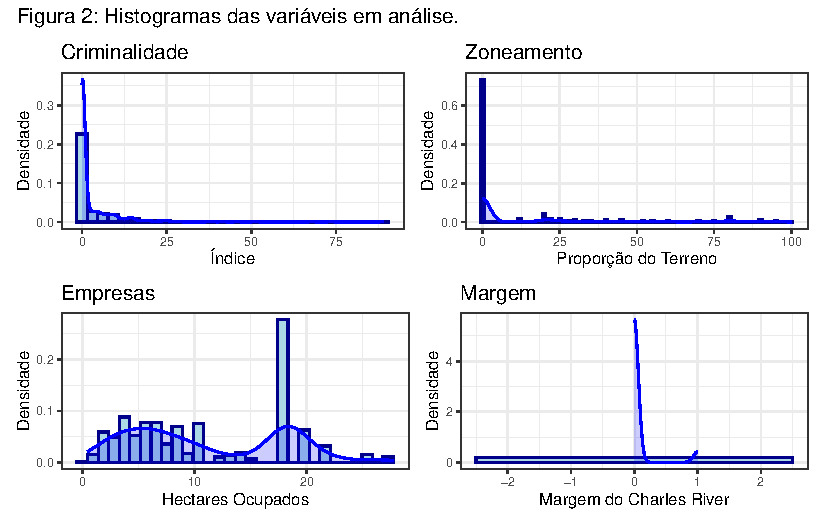
\includegraphics{Parte-1_files/figure-pdf/unnamed-chunk-3-1.pdf}

}

\end{figure}

\begin{figure}[H]

{\centering 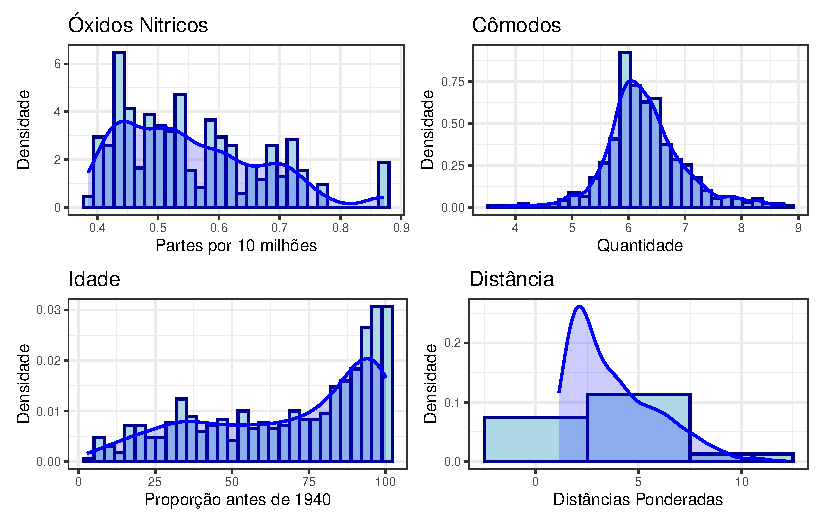
\includegraphics{Parte-1_files/figure-pdf/unnamed-chunk-3-2.pdf}

}

\end{figure}

\begin{figure}[H]

{\centering 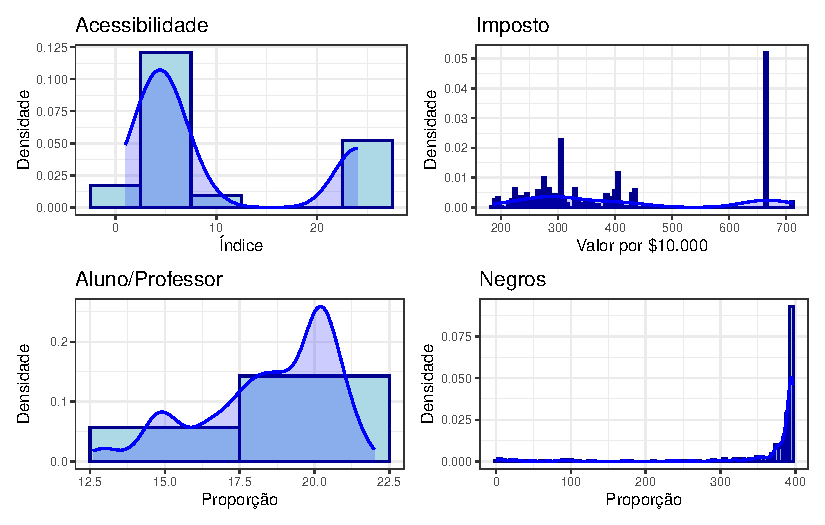
\includegraphics{Parte-1_files/figure-pdf/unnamed-chunk-3-3.pdf}

}

\end{figure}

\begin{figure}[H]

{\centering 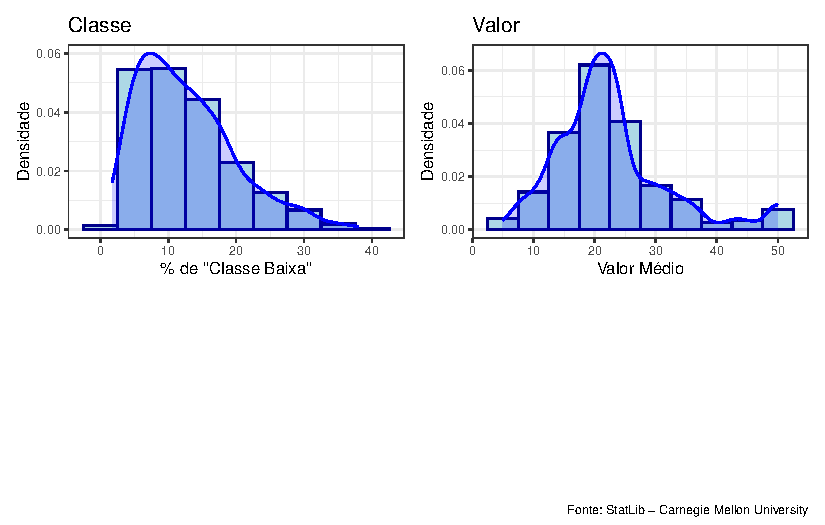
\includegraphics{Parte-1_files/figure-pdf/unnamed-chunk-3-4.pdf}

}

\end{figure}

\begin{figure}[H]

{\centering 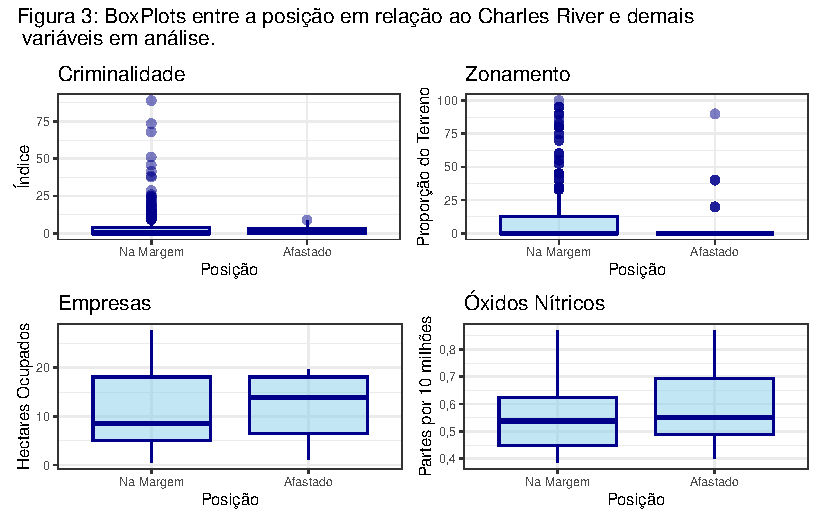
\includegraphics{Parte-1_files/figure-pdf/unnamed-chunk-4-1.pdf}

}

\end{figure}

\begin{figure}[H]

{\centering 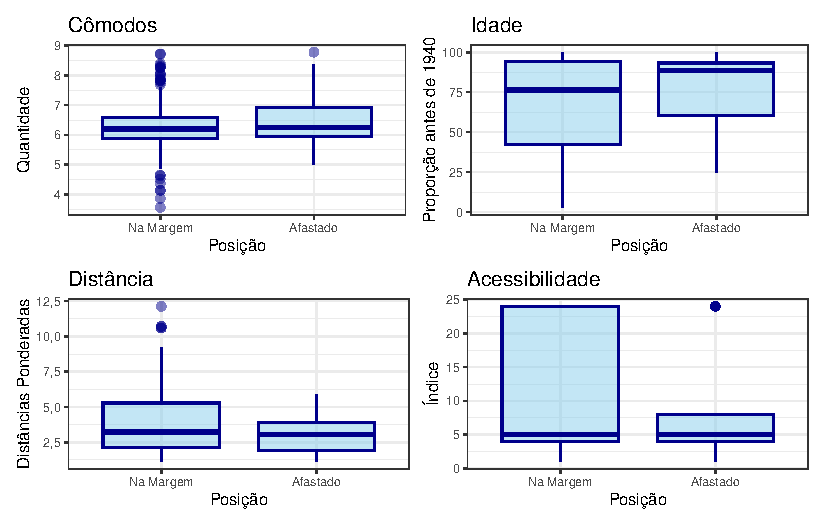
\includegraphics{Parte-1_files/figure-pdf/unnamed-chunk-4-2.pdf}

}

\end{figure}

\begin{figure}[H]

{\centering 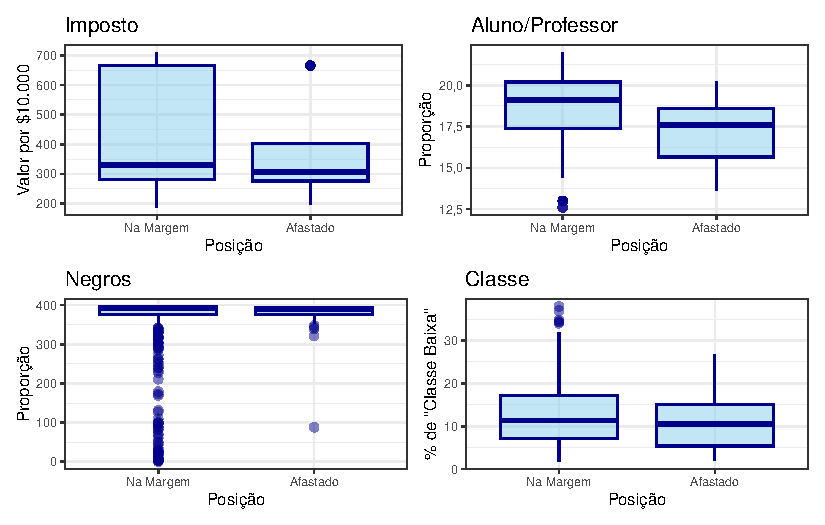
\includegraphics{Parte-1_files/figure-pdf/unnamed-chunk-4-3.pdf}

}

\end{figure}

\begin{figure}[H]

{\centering 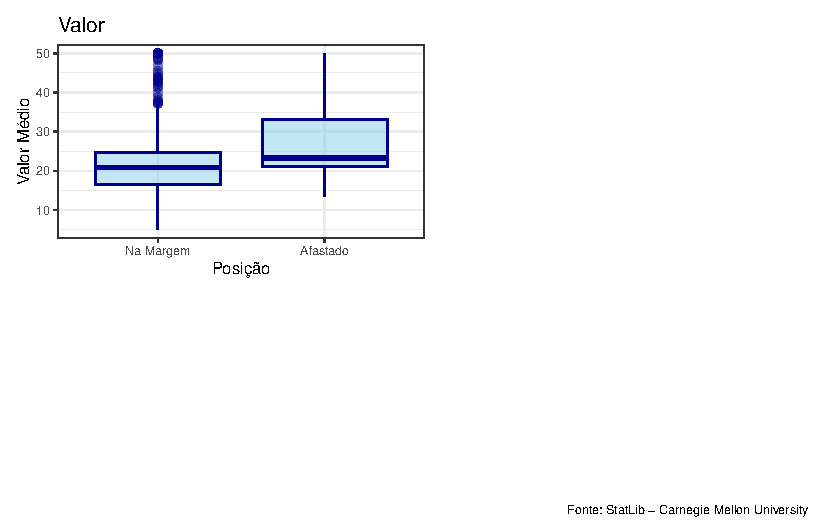
\includegraphics{Parte-1_files/figure-pdf/unnamed-chunk-4-4.pdf}

}

\end{figure}

\begin{figure}[H]

{\centering 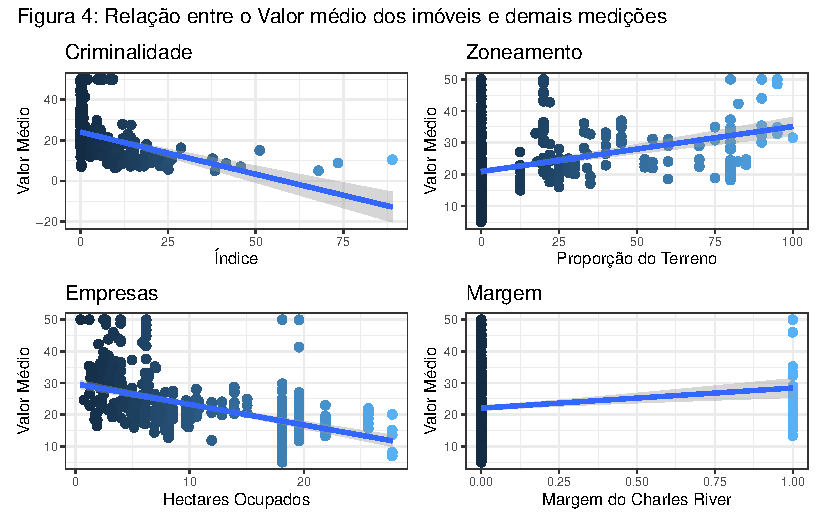
\includegraphics{Parte-1_files/figure-pdf/unnamed-chunk-5-1.pdf}

}

\end{figure}

\begin{figure}[H]

{\centering 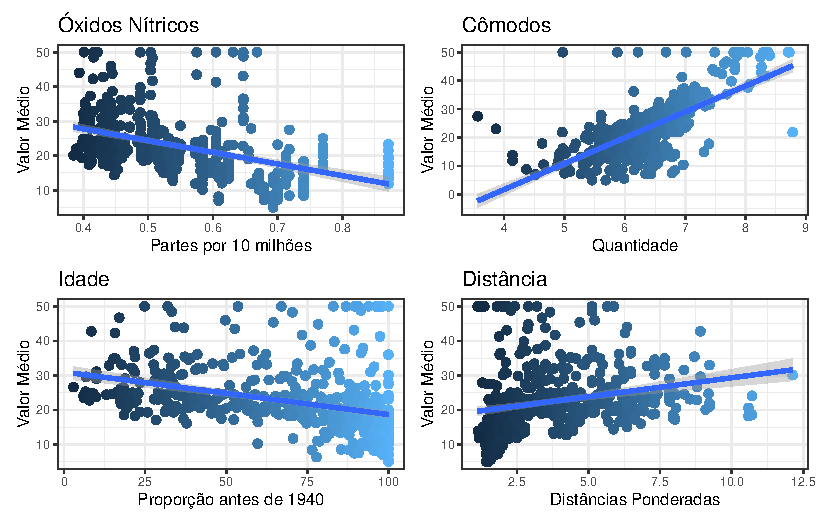
\includegraphics{Parte-1_files/figure-pdf/unnamed-chunk-5-2.pdf}

}

\end{figure}

\begin{figure}[H]

{\centering 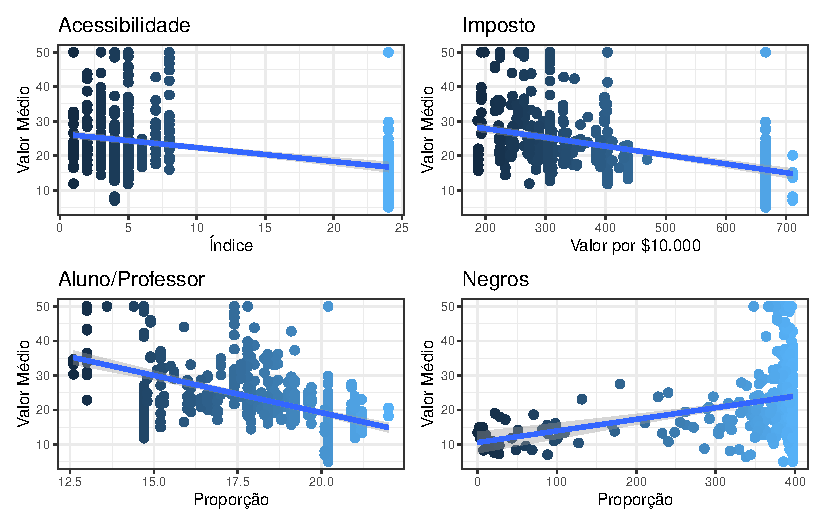
\includegraphics{Parte-1_files/figure-pdf/unnamed-chunk-5-3.pdf}

}

\end{figure}

\begin{figure}[H]

{\centering 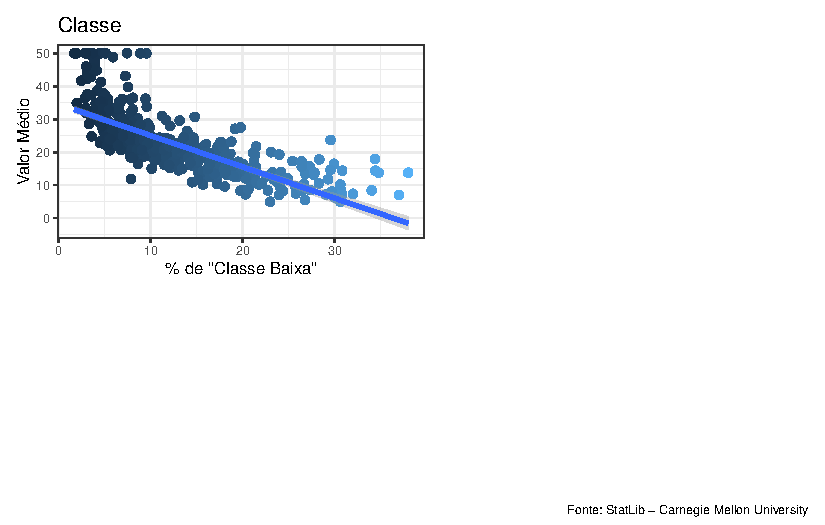
\includegraphics{Parte-1_files/figure-pdf/unnamed-chunk-5-4.pdf}

}

\end{figure}

\begin{table}[H]

\caption{Valores dos modelos de regressão linear simples.}
\centering
\begin{tabular}[t]{l|c|c|c|c|c|c|c}
\hline
  & CRIM & ZN & INDUS & CHAS & NOX & RM & AGE\\
\hline
$\beta_0$ & 24,033 & 20,918 & 29,755 & 22,094 & 41,346 & -34,671 & 30,979\\
\hline
$\sigma_0$ & 0,409 & 0,425 & 0,683 & 0,418 & 1,811 & 2,650 & 0,999\\
\hline
$\beta_1$ & -0,415 & 0,142 & -0,648 & 6,346 & -33,916 & 9,102 & -0,123\\
\hline
$\sigma_1$ & 0,044 & 0,016 & 0,052 & 1,588 & 3,196 & 0,419 & 0,013\\
\hline
p-valor & 0,000 & 0,000 & 0,000 & 0,000 & 0,000 & 0,000 & 0,000\\
\hline
$\hat \rho$ & 0,151 & 0,130 & 0,234 & 0,031 & 0,183 & 0,484 & 0,142\\
\hline
\end{tabular}
\end{table}

\begin{table}[H]
\centering
\begin{tabular}[t]{l|c|c|c|c|c|c}
\hline
  & DIS & RAD & TAX & PTRATIO & B & LSTAT\\
\hline
$\beta_0$ & 18,390 & 26,382 & 32,971 & 62,345 & 10,551 & 34,554\\
\hline
$\sigma_0$ & 0,817 & 0,562 & 0,948 & 3,029 & 1,557 & 0,563\\
\hline
$\beta_1$ & 1,092 & -0,403 & -0,026 & -2,157 & 0,034 & -0,950\\
\hline
$\sigma_1$ & 0,188 & 0,043 & 0,002 & 0,163 & 0,004 & 0,039\\
\hline
p-valor & 0,000 & 0,000 & 0,000 & 0,000 & 0,000 & 0,000\\
\hline
$\hat \rho$ & 0,062 & 0,146 & 0,220 & 0,258 & 0,111 & 0,544\\
\hline
\end{tabular}
\end{table}

\begin{figure}[H]

{\centering 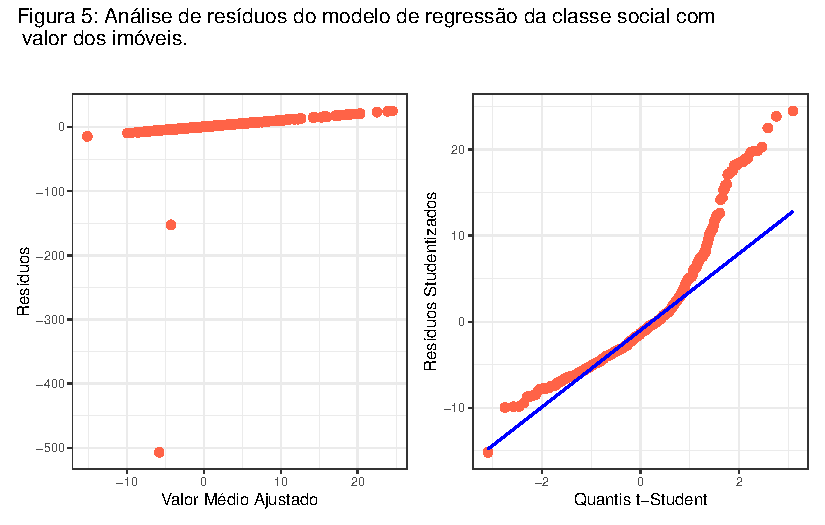
\includegraphics{Parte-1_files/figure-pdf/unnamed-chunk-7-1.pdf}

}

\end{figure}

\hypertarget{testes-de-diagnuxf3stico}{%
\subsection{Testes de diagnóstico}\label{testes-de-diagnuxf3stico}}

Pode-se ainda utilizar um conjunto de testes de diagnóstico para
confirmar este novo teste de significância. Como:

\begin{itemize}
\tightlist
\item
  Teste de Kolmogorov-Smirnov\\
\item
  Teste de Shapiro-Wilks\\
\item
  Teste de Goldfeld-Quandt\\
\item
  Teste de Breush-Pagan\\
\item
  Teste de Park\\
\item
  Teste F para linearidade\\
\item
  Teste para avaliação da independência dos resíduos\\
\end{itemize}

\hypertarget{teste-de-kolmogorov-smirnov}{%
\paragraph{Teste de
Kolmogorov-Smirnov}\label{teste-de-kolmogorov-smirnov}}

Avalia o grau de concordância entre a distribuição de um conjunto de
valores observados e determinada distribuição teórica. Consiste em
comparar a distribuição de frequência acumulada da distribuição teórica
com aquela observada. Realizado o teste obteve-se um p-valor de
aproximadamente 0, o que inviabiliza rejeitar a hipótese de que haja
normalidade entre os dados, com um grau de confiabilidade minimamente
razoável.

\hypertarget{teste-de-shapiro-wilks}{%
\paragraph{Teste de Shapiro-Wilks}\label{teste-de-shapiro-wilks}}

O teste de Shapiro-Wilks é um procedimento alternativo ao teste de
Kolmogorov-Smirnov para avaliar normalidade. Realizado o teste obteve-se
um p-valor de aproximadamente 0, o que, semelhantemente, inviabiliza
rejeitar a hipótese de que haja normalidade entre os dados, com um grau
de confiabilidade minimamente razoável.

\hypertarget{teste-de-goldfeld-quandt}{%
\paragraph{Teste de Goldfeld-Quandt}\label{teste-de-goldfeld-quandt}}

Esse teste envolve o ajuste de dois modelos de regressão, separando-se
as observações das duas extremidades da distribuição da variável
dependente. Realizado o teste obteve-se um p-valor de aproximadamente
0.058, o que demanda rejeitar a hipótese de que haja homocedasticidade
entre os dados, com um grau de confiabilidade de 95\%. Entretanto, como
o p-valor obtido é próximo do necessário para a rejeição da hipotese
nula, cabe um novo teste para a confirmação do resultado obtido.

\hypertarget{teste-de-breush-pagan}{%
\paragraph{Teste de Breush-Pagan}\label{teste-de-breush-pagan}}

Esse teste é baseado no ajuste de um modelo de regressão em que a
variável dependente é definida pelos resíduos do modelo de interesse. Se
grande parte da variabilidade dos resíduos não é explicada pelo modelo,
então rejeita-se a hipótese de homocedasticidade. Realizado o teste
obteve-se um p-valor de aproximadamente 0, desta foram deve-se rejeitar
a hipótese de que haja homocedasticidade entre os dados, com um grau de
confiabilidade de 95\%.

\hypertarget{teste-de-park}{%
\paragraph{Teste de Park}\label{teste-de-park}}

Esse teste é baseado no ajuste de um modelo de regressão em que a
variável dependente é definida pelos quadrados dos resíduos do modelo de
interesse. Nesse caso, se \(\beta_1\) diferir significativamente de
zero, rejeita-se a hipótese de homocedasticidade. O valor de \(\beta_1\)
obtido no teste foi de -1.962 com p-valor de aproximadamente 0. Por esse
teste não se deve rejeitar a hipótese de homocedasticidade, com
confiabilidade de 95\%.

\hypertarget{teste-f-para-linearidade}{%
\paragraph{Teste F para linearidade}\label{teste-f-para-linearidade}}

O teste da falta de ajuste permite testar formalmente a adequação do
ajuste do modelo de regressão. Neste ponto assume-se que os pressupostos
de normalidade, variância constante e independência são satisfeitos,
como demosntrado pelos testes realizados. A ideia central para testar a
linearidade é decompor SQRes em duas partes: erro puro e falta de ajuste
que vão contribuir para a definição da estatística de teste F. Realizado
o teste obteve-se um valore de p-valor igual a 0.289, o que demanda a
rejeição da hipótese que há uma relação linear entre as variáveis.

\hypertarget{teste-para-avaliauxe7uxe3o-da-independuxeancia-dos-resuxedduos}{%
\paragraph{Teste para avaliação da independência dos
resíduos}\label{teste-para-avaliauxe7uxe3o-da-independuxeancia-dos-resuxedduos}}

Tendo em vista, o resultado obtido no teste anterior esse teste pode
esclarecer ainda mais o ajuste do modelo.\\
O teste para avaliação da independência dos resíduos é utilizado para
detectar a presença de autocorrelação provenientes de análise de
regressão. Realizando o teste obteve-se um valor de p-valor
aproximadadente igual a 0, indicando que se deve rejeitar a hipotese que
não existe correlação serial entre os dados, com uma confiança de 95\%.

\hypertarget{conclusuxe3o}{%
\section{Conclusão}\label{conclusuxe3o}}

\hypertarget{referuxeancias}{%
\subsection{Referências}\label{referuxeancias}}

Harrison, David \& Rubinfeld, Daniel. (1978). Hedonic housing prices and
the demand for clean air. Journal of Environmental Economics and
Management. 5. 81-102. 10.1016/0095-0696(78)90006-2.

Belsley, David A. \& Kuh, Edwin. \& Welsch, Roy E. (1980). Regression
diagnostics: identifying influential data and sources of collinearity.
New York: Wiley.



\end{document}
